\documentclass[../main.tex]{subfiles}


\begin{document}

\chapter{MATLAB Fundamentals}




\begin{center}
\Large{\textbf{CHAPTER OBJECTIVES}}
\end{center}

\normalsize{The primary objective of this chapter is to provide an introduction and overview of
how MATLAB's calculator mode is used to implement interactive computations.
Specific objectives and topics covered are}
'
\begin{itemize}


	\item Learning how real and complex numbers are assigned to variables
	\item  Learning how vectors and matrices are assigned values using simple assignment,
the colon operator, and the linspace and logspace functions.
\item  Understanding the priority rules for constructing mathematical expressions.
\item  Gaining a general understanding of built-in functions and how you can learn more
about them with MATLAB's Help facilities.
\item  Learning how to use vectors to create a simple line plot based on an equation.
\end{itemize}
\Large{YOU'VE GOT A PROBLEM}
\normalsize

n Chap. 1, we used a force balance to determine the terminal velocity of a free-falling
object like a bungee jumper.

$$v_t=\sqrt{\dfrac{gm}{c_d}}  $$

where $v_t =$ terminal velocity (m/s), $g =$ gravitational acceleration ($m/s2$
), $m =$ mass (kg),
and $c_d =$ a drag coefficient (kg/m). Aside from predicting the terminal velocity, this equation can also be rearranged to compute the drag coefficient
 
\begin{equation}
	\tag{2.1}
	c_d = \dfrac{mg}{v^2_t}
\end{equation} 



	\begin{table}[H]
		\centering
		\caption{Data for the mass and associated terminal velocities of a number of jumpers.}
		\begin{tabular}{cccccccc}
			\hline
			$m, kg$ 	&83.6 &60.2 &72.1 &91.1 &92.9 &65.3 &80.9\\
			$v_t, m/s$ &53.4 &48.5 &50.9 &55.7 &54 &47.7 &51.1\\
			\hline
			
		\end{tabular}
	\end{table}


	Thus, if we measure the terminal velocity of a number of jumpers of known mass, this
equation provides a means to estimate the drag coefficient. The data in Table 2.1 were collected for this purpose.


In this chapter, we will learn how MATLAB can be used to analyze such data. Beyond
showing how MATLAB can be employed to compute quantities like drag coefficients, we
will also illustrate how its graphical capabilities provide additional insight into such analyses.


\section{THE MATLAB ENVIRONMENT}


MATLAB is a computer program that provides the user with a convenient environment for
performing many types of calculations. In particular, it provides a very nice tool to implement numerical methods.


The most common way to operate MATLAB is by entering commands one at a time in
the command window. In this chapter, we use this interactive or calculator mode to introduce you to common operations such as performing calculations and creating plots. In
Chap. 3, we show how such commands can be used to create MATLAB programs.


One further note. This chapter has been written as a hands-on exercise. That is, you
should read it while sitting in front of your computer. The most efficient way to become
proficient is to actually implement the commands on MATLAB as you proceed through the
following material.


MATLAB uses three primary windows:
\begin{itemize}
	\item Command window. Used to enter commands and data.
	\item Graphics window. Used to display plots and graphs.
	\item Edit window. Used to create and edit M-files
\end{itemize}

In this chapter, we will make use of the command and graphics windows. In Chap. 3 we
will use the edit window to create M-files.


After starting MATLAB, the command window will open with the command prompt
being displayed



\begin{lstlisting}[frame=none, numbers=none]
	>>
\end{lstlisting}

MATLAB will display the result
	
\begin{lstlisting}[frame=none, numbers=none]
	ans=
		39
\end{lstlisting}

Notice that MATLAB has automatically assigned the answer to a variable, ans. Thus, you
could now use ans in a subsequent calculation:

\begin{lstlisting}[frame=none, numbers=none]
	ans + 11
\end{lstlisting}

with the result

\begin{lstlisting}[frame=none, numbers=none]
	ans=
		50
\end{lstlisting}

MATLAB assigns the result to ans whenever you do not explicitly assign the calculation
to a variable of your own choosing.

\section{ASSIGNMENT}

Assignment refers to assigning values to variable names. This results in the storage of the
values in the memory location corresponding to the variable name.

\subsection{Scalars}
The assignment of values to scalar variables is similar to other computer languages.
Try typing
\begin{lstlisting}[frame=none, numbers=none]
	>> a = 4
\end{lstlisting}

Note how the assignment echo prints to confirm what you have done:
\begin{lstlisting}[frame=none, numbers=none]
	a = 
		4
\end{lstlisting}

Echo printing is a characteristic of MATLAB. It can be suppressed by terminating the command line with the semicolon (;) character. Try typing
\begin{lstlisting}[frame=none, numbers=none]
	>> A = 6;
\end{lstlisting}

You can type several commands on the same line by separating them with commas or
semicolons. If you separate them with commas, they will be displayed, and if you use the
semicolon, they will not. For example,

\begin{lstlisting}[frame=none, numbers=none]
	>> a = 4,A = 6;x = 1;
	a =
		4
\end{lstlisting}
MATLAB treats names in a case-sensitive manner—that is, the variable a is not the
same as A. To illustrate this, enter

\begin{lstlisting}[frame=none, numbers=none]
	>> a
\end{lstlisting}
and then enter

\begin{lstlisting}[frame=none, numbers=none]
	>> A
\end{lstlisting}
See how their values are distinct. They are distinct names.

We can assign complex values to variables, since MATLAB handles complex arithmetic automatically. The unit imaginary number √
-1 is preassigned to the variable i.
Consequently, a complex value can be assigned simply as in
\begin{lstlisting}[frame=none, numbers=none]
	>> x = 2+i*4
	x =
		2.0000 + 4.0000i
\end{lstlisting}

It should be noted that MATLAB allows the symbol j to be used to represent the unit imaginary number for input. However, it always uses an i for display. For example,
\begin{lstlisting}[frame=none, numbers=none]
	>> x = 2+j*4
	x =
		2.0000 + 4.0000i
\end{lstlisting}

There are several predefined variables, for example, pi.
\begin{lstlisting}[frame=none, numbers=none]
	>> pi
	ans =
		3.1416
\end{lstlisting}

Notice how MATLAB displays four decimal places. If you desire additional precision,
enter the following:
\begin{lstlisting}[frame=none, numbers=none]
	>> format long
\end{lstlisting}
Now when pi is entered the result is displayed to 15 significant figures:
\begin{lstlisting}[frame=none, numbers=none]
	>> pi
	ans =
		3.14159265358979
\end{lstlisting}
To return to the four decimal version, type
\begin{lstlisting}[frame=none, numbers=none]
	>> format short
\end{lstlisting}
The following is a summary of the format commands you will employ routinely in engineering and scientific calculations. They all have the syntax: format type.

\begin{table}[h]
	\centering
	\begin{tabular}{ l l l }
		\hline
		\textbf{type} &\textbf{Result} &\textbf{Example}\\
		\hline
		short 	&	Scaled fixed-point format with 5 digits &3.1416\\
		long	&	 Scaled fixed-point format with 15 digits for double and 7 digits for single& 3.14159265358979\\
		short e &		Floating-point format with 5 digits &3.1416e+000\\
		long e 	&	Floating-point format with 15 digits for double and 7 digits for single &3.141592653589793e+000\\
		short g	&	 Best of fixed- or floating-point format with 5 digits& 3.1416\\
		long g 	&	Best of fixed- or floating-point format with 15 digits for doubleand 7 digits for single &3.14159265358979\\
		short eng	& Engineering format with at least 5 digits and a power that is a multiple of 3 &3.1416e+000\\
		long eng 	&Engineering format with exactly 16 significant digits and a powerthat is a multiple of 3 &3.14159265358979e+000\\
		bank 	&	Fixed dollars and cents &3.14\\
		\hline
	\end{tabular}
\end{table}


\subsection{Arrays, Vectors and Matrices}

An array is a collection of values that are represented by a single variable name. One-dimensional arrays are called vectors and two-dimensional arrays are called matrices. The
scalars used in Section 2.2.1 are actually matrices with one row and one column.
Brackets are used to enter arrays in the command mode. For example, a row vector can
be assigned as follows:
\begin{lstlisting}[frame=none, numbers=none]
	>> format long
\end{lstlisting}
>> a = [1 2 3 4 5]
a =
1 2 3 4 5
Note that this assignment overrides the previous assignment of a = 4.
In practice, row vectors are rarely used to solve mathematical problems. When we
speak of vectors, we usually refer to column vectors, which are more commonly used. A
column vector can be entered in several ways. Try them.
\begin{lstlisting}[frame=none, numbers=none]
	>> b = [2;4;6;8;10]
\end{lstlisting}
or
\begin{lstlisting}[frame=none, numbers=none]
	>> b = [2
			4
			6
			8
			10]
\end{lstlisting}
or, by transposing a row vector with the ' operator,
\begin{lstlisting}[frame=none, numbers=none]
	>> b = [2 4 6 8 10]'

\end{lstlisting}
The result in all three cases will be
\begin{lstlisting}[frame=none, numbers=none]
	b =
		2
		4
		6
		8
		10
\end{lstlisting}
A matrix of values can be assigned as follows:
\begin{lstlisting}[frame=none, numbers=none]
	>> A = [1 2 3; 4 5 6; 7 8 9]
	A =
		1 2 3
		4 5 6
		7 8 9
\end{lstlisting}
In addition, the Enter key (carriage return) can be used to separate the rows. For example,
in the following case, the Enter key would be struck after the 3, the 6 and the ] to assign the
matrix:
\begin{lstlisting}[frame=none, numbers=none]
	>> A = 
			[1 2 3
			4 5 6
			7 8 9]

\end{lstlisting}
Finally, we could construct the same matrix by concatenating (i.e., joining) the vectors
representing each column:
\begin{lstlisting}[frame=none, numbers=none]
	>> A = [[1 4 7]' [2 5 8]' [3 6 9]']
\end{lstlisting}
At any point in a session, a list of all current variables can be obtained by entering the
who command:
\begin{lstlisting}[frame=none, numbers=none]
	>> who

	Your variables are:
	A a ans b x
\end{lstlisting}
or, with more detail, enter the whos command:
\begin{lstlisting}[frame=none, numbers=none]
	>> whos

	Name		Size 		Bytes	 Class
	A 			3x3 		72		 double array
	a 			1x5 		40		 double array
	ans 		1x1 		8		 	double array
	b 			5x1 		40		 double array
	x 			1x1 		16		 double array (complex)
	Grand total is 21 elements using 176 bytes
\end{lstlisting}
Note that subscript notation can be used to access an individual element of an array.
For example, the fourth element of the column vector b can be displayed as
\begin{lstlisting}[frame=none, numbers=none]
	>> b(4)

	ans =
		8
\end{lstlisting}
For an array, A(m,n) selects the element in mth row and the nth column. For example,
\begin{lstlisting}[frame=none, numbers=none]
	>> A(2,3)

	ans =
		6
\end{lstlisting}
There are several built-in functions that can be used to create matrices. For example,
the ones and zeros functions create vectors or matrices filled with ones and zeros,
respectively. Both have two arguments, the first for the number of rows and the second for
the number of columns. For example, to create a 2 $\times$  3 matrix of zeros:
\begin{lstlisting}[frame=none, numbers=none]
	>> E = zeros(2,3)

	E =
		0 0 0
		0 0 0
\end{lstlisting}
Similarly, the ones function can be used to create a row vector of ones:
\begin{lstlisting}[frame=none, numbers=none]
	>> u = ones(1,3)

	u =
		1 1 1
\end{lstlisting}

\subsection{The Colon Operator}\

The colon operator is a powerful tool for creating and manipulating arrays. If a colon is
used to separate two numbers, MATLAB generates the numbers between them using an
increment of one:
\begin{lstlisting}[frame=none, numbers=none]
	>> t = 1:5

	t =
		1 2 3 4 5
\end{lstlisting}
If colons are used to separate three numbers, MATLAB generates the numbers between the
first and third numbers using an increment equal to the second number:
\begin{lstlisting}[frame=none, numbers=none]
	>> t = 1:0.5:3

	t =
		1.0000 1.5000 2.0000 2.5000 3.0000
\end{lstlisting}
Note that negative increments can also be used
\begin{lstlisting}[frame=none, numbers=none]
	>> t = 10:-1:5

	t =
		10 9 8 7 6 5
\end{lstlisting}
Aside from creating series of numbers, the colon can also be used as a wildcard to select the individual rows and columns of a matrix. When a colon is used in place of a specific subscript, the colon represents the entire row or column. For example, the second row
of the matrix A can be selected as in
\begin{lstlisting}[frame=none, numbers=none]
	>> A(2,:)

	ans =
		4 5 6
\end{lstlisting}
We can also use the colon notation to selectively extract a series of elements from
within an array. For example, based on the previous definition of the vector t:
\begin{lstlisting}[frame=none, numbers=none]
	>> t(2:4)

	ans =
		9 8 7
\end{lstlisting}
Thus, the second through the fourth elements are returned.

\subsection{The linspace and logspace Functions}

The linspace and logspace functions provide other handy tools to generate vectors of
spaced points. The linspace function generates a row vector of equally spaced points. It
has the form
\begin{lstlisting}[frame=none, numbers=none]
	linspace(x1, x2, n)
\end{lstlisting}
which generates n points between x1 and x2. For example
\begin{lstlisting}[frame=none, numbers=none]
	>> linspace(0,1,6)

	ans =
		0 0.2000 0.4000 0.6000 0.8000 1.0000
\end{lstlisting}
If the n is omitted, the function automatically generates 100 points.
The logspace function generates a row vector that is logarithmically equally spaced.
It has the form
\begin{lstlisting}[frame=none, numbers=none]
	logspace(x1, x2, n)
\end{lstlisting}
which generates n logarithmically equally spaced points between decades 10x1 and 10x2.
For example,
\begin{lstlisting}[frame=none, numbers=none]
	>> logspace(-1,2,4)

	ans =
		0.1000 1.0000 10.0000 100.0000
\end{lstlisting}
If n is omitted, it automatically generates 50 points.

\subsection{Character Strings}

Aside from numbers, alphanumeric information or character strings can be represented by
enclosing the strings within single quotation marks. For example,
\begin{lstlisting}[frame=none, numbers=none]
	>> f = 'Miles ';
	>> s = 'Davis';	
\end{lstlisting}
Each character in a string is one element in an array. Thus, we can concatenate (i.e., paste
together) strings as in
\begin{lstlisting}[frame=none, numbers=none]
	>> x = [f s]

	x =
	Miles Davis
\end{lstlisting}
Note that very long lines can be continued by placing an ellipsis (three consecutive
periods) at the end of the line to be continued. For example, a row vector could be entered as
\begin{lstlisting}[frame=none, numbers=none]
	>> a = [1 2 3 4 5 ...
	6 7 8]

	a =
		1 2 3 4 5 6 7 8
\end{lstlisting}
However, you cannot use an ellipsis within single quotes to continue a string. To enter a
string that extends beyond a single line, piece together shorter strings as in
\begin{lstlisting}[frame=none, numbers=none]
	>> quote = ['Any fool can make a rule,' ...
	' and any fool will mind it']

	quote =
	Any fool can make a rule, and any fool will mind it
\end{lstlisting}


\section{MATHEMATICAL OPERATIONS}

Operations with scalar quantities are handled in a straightforward manner, similar to other
computer languages. The common operators, in order of priority, are

\begin{table}[H]
	\centering
	\begin{tabular}{ll}
		\hline
			& Exponentiation\\
		$ - $ &Negation\\
		$ \ast  \ \setminus $ &Multiplication and division\\
		$ \setminus$ &Left division\\
		$ + \ - $ &Addition and subtraction\\
		\hline
	\end{tabular}
\end{table}



These operators will work in calculator fashion. Try
\begin{lstlisting}[frame=none, numbers=none]
	>> 2*pi

	ans =
		6.2832
\end{lstlisting}
Also, scalar real variables can be included:
\begin{lstlisting}[frame=none, numbers=none]
	>> y = pi/4;
	>> y ^ 2.45

	ans =
		0.5533
\end{lstlisting}
Results of calculations can be assigned to a variable, as in the next-to-last example, or simply displayed, as in the last example.
As with other computer calculation, the priority order can be overridden with parentheses. For example, because exponentiation has higher priority then negation, the following result would be obtained:
\begin{lstlisting}[frame=none, numbers=none]
	>> y = -4 ^ 2
	
	y =
		-16
\end{lstlisting}
Thus, 4 is first squared and then negated. Parentheses can be used to override the priorities
as in
\begin{lstlisting}[frame=none, numbers=none]
	>> y = (-4) ^ 2

	y =
		16
\end{lstlisting}


Calculations can also involve complex quantities. Here are some examples that use the
values of $x (2 + 4i)$ and $y(16)$ defined previously:
\begin{lstlisting}[frame=none, numbers=none]
	>> 3 * x

	ans =
		6.0000 + 12.0000i
	>> 1 / x

	ans =
		0.1000 - 0.2000i
	>> x ^ 2

	ans =
		-12.0000 + 16.0000i
	>> x + y

	ans =
		18.0000 + 4.0000i
\end{lstlisting}
The real power of MATLAB is illustrated in its ability to carry out vector-matrix
calculations. Although we will describe such calculations in detail in Chap. 8, it is worth
introducing some examples here.
The inner product of two vectors (dot product) can be calculated using the * operator,
\begin{lstlisting}[frame=none, numbers=none]
	>> a * b
	ans =
		110
\end{lstlisting}
and likewise, the outer product
\begin{lstlisting}[frame=none, numbers=none]
	>> b * a

	ans =
		2 	4 	6 	8 	10
		4 	8 	12 	16 	20
		6 	12 	18 	24 	30
		8 	16 	24 	32 	40
		10 	20 	30 	40 	50
\end{lstlisting}
To further illustrate vector-matrix multiplication, first redefine a and b:
\begin{lstlisting}[frame=none, numbers=none]
	>> a = [1 2 3];
\end{lstlisting}
and
\begin{lstlisting}[frame=none, numbers=none]
	>> b = [4 5 6]';
\end{lstlisting}
Now, try
\begin{lstlisting}[frame=none, numbers=none]
	>> a * A

	ans =
		30 36 42
\end{lstlisting}

or
\begin{lstlisting}[frame=none, numbers=none]
	>> A * b
	ans =
		32
		77
		122
\end{lstlisting}
Matrices cannot be multiplied if the inner dimensions are unequal. Here is what happens
when the dimensions are not those required by the operations. Try
\begin{lstlisting}[frame=none, numbers=none]
	>> A * a
\end{lstlisting}
MATLAB automatically displays the error message:
\begin{lstlisting}[frame=none, numbers=none]
	??? Error using ==> mtimes
	Inner matrix dimensions must agree.	
\end{lstlisting}
Matrix-matrix multiplication is carried out in likewise fashion:
\begin{lstlisting}[frame=none, numbers=none]
	>> A * A

	ans =
		30	36 	42
		66	81 	96
		102 126	150
\end{lstlisting}
Mixed operations with scalars are also possible:
\begin{lstlisting}[frame=none, numbers=none]
	>> A/pi

	ans =
		0.3183 0.6366 0.9549
		1.2732 1.5915 1.9099
		2.2282 2.5465 2.8648
\end{lstlisting}
We must always remember that MATLAB will apply the simple arithmetic operators
in vector-matrix fashion if possible. At times, you will want to carry out calculations item
by item in a matrix or vector. MATLAB provides for that too. For example,
\begin{lstlisting}[frame=none, numbers=none]
	>> A^2

	ans =
		30 	36 	42
		66 	81 	96
		102	126	150
\end{lstlisting}
results in matrix multiplication of A with itself.


What if you want to square each element of A? That can be done with
\begin{lstlisting}[frame=none, numbers=none]
	>> A.^2

	ans =
		1 	4 	9
		16 	25 	36
		49 	64 	81
\end{lstlisting}
The \. preceding the \^ operator signifies that the operation is to be carried out element by
element. The MATLAB \textsl{manual calls these array operations.} They are also often referred
to as \textsl{element-by-element operations.}


MATLAB contains a helpful shortcut for performing calculations that you've already
done. Press the up-arrow key. You should get back the last line you typed in.
\begin{lstlisting}[frame=none, numbers=none]
	>> A.^2
\end{lstlisting}
Pressing Enter will perform the calculation again. But you can also edit this line. For
example, change it to the line below and then press Enter.
\begin{lstlisting}[frame=none, numbers=none]
	>> A.^3

	ans =
		1 	8 	27
		64 	125	216
		343	512	729
\end{lstlisting}
Using the up-arrow key, you can go back to any command that you entered. Press the uparrow until you get back the line
\begin{lstlisting}[frame=none, numbers=none]
	>> b * a
\end{lstlisting}
Alternatively, you can type b and press the up-arrow once and it will automatically bring
up the last command beginning with the letter b. The up-arrow shortcut is a quick way to
fix errors without having to retype the entire line.


\section{USE OF BUILT-IN FUNCTIONS}

MATLAB and its Toolboxes have a rich collection of built-in functions. You can use online
help to find out more about them. For example, if you want to learn about the log function,
type in
\begin{lstlisting}[frame=none, numbers=none]
	>> help log

	LOG Natural logarithm.
		LOG(X) is the natural logarithm of the elements of X.
		Complex results are produced if X is not positive.

		ee also LOG2, LOG10, EXP, LOGM.
\end{lstlisting}
For a list of all the elementary functions, type
\begin{lstlisting}[frame=none, numbers=none]
	>> help elfun
\end{lstlisting}
One of their important properties of MATLAB's built-in functions is that they will operate directly on vector and matrix quantities. For example, try
\begin{lstlisting}[frame=none, numbers=none]
	>> log(A)
	ans =
		0 		0.6931	1.0986
		1.3863 	1.6094	1.7918
		1.9459 	2.0794	2.1972
\end{lstlisting}
and you will see that the natural logarithm function is applied in array style, element by
element, to the matrix A. Most functions, such as sqrt, abs, sin, acos, tanh, and exp, operate 
in array fashion. Certain functions, such as exponential and square root, have matrix

definitions also. MATLAB will evaluate the matrix version when the letter m is appended to
the function name. Try
\begin{lstlisting}[frame=none, numbers=none]
	>> sqrtm(A)

	ans =
		0.4498 + 0.7623i 0.5526 + 0.2068i 0.6555 - 0.3487i
		1.0185 + 0.0842i 1.2515 + 0.0228i 1.4844 - 0.0385i
		1.5873 - 0.5940i 1.9503 - 0.1611i 2.3134 + 0.2717i
\end{lstlisting}

There are several functions for rounding. For example, suppose that we enter a vector:
\begin{lstlisting}[frame=none, numbers=none]
	>> E = [-1.6 -1.5 -1.4 1.4 1.5 1.6];
\end{lstlisting}
The round function rounds the elements of E to the nearest integers:
\begin{lstlisting}[frame=none, numbers=none]
	>> round(E)

	ans =
		-2 -2 -1 1 2 2
\end{lstlisting}
The ceil (short for ceiling) function rounds to the nearest integers toward infinity:
\begin{lstlisting}[frame=none, numbers=none]
	>> ceil(E)

	ans =
		-1 -1 -1 2 2 2
\end{lstlisting}
The floor function rounds down to the nearest integers toward minus infinity:
\begin{lstlisting}[frame=none, numbers=none]
	>> floor(E)

	ans =
		-2 -2 -2 1 1 1
\end{lstlisting}
There are also functions that perform special actions on the elements of matrices and
arrays. For example, the sum function returns the sum of the elements:
\begin{lstlisting}[frame=none, numbers=none]
	>> F = [3 5 4 6 1];

	>> sum(F)

	ans =
		19
\end{lstlisting}
In a similar way, it should be pretty obvious what's happening with the following commands:
\begin{lstlisting}[frame=none, numbers=none]
	>> min(F),max(F),mean(F),prod(F),sort(F)

	ans =
		1
	ans =
		6
	ans =
		3.8000
	ans =
		360
	ans =

		1 3 4 5 6
\end{lstlisting}


A common use of functions is to evaluate a formula for a series of arguments. Recall
that the velocity of a free-falling bungee jumper can be computed with [Eq. (1.9)]:

$$ v= \sqrt{\dfrac{gm}{c_d}}tanh \left( \sqrt{\dfrac{gc_d}{m}}t \right) $$

where v is velocity (m/s), g is the acceleration due to gravity (9.81 $m/s^2$
), m is mass (kg),
cd is the drag coefficient (kg/m), and t is time (s).
Create a column vector t that contains values from 0 to 20 in steps of 2:
\begin{lstlisting}[frame=none, numbers=none]
	>> t = [0:2:20]'
	t =
		0
		2
		4
		6
		8
		10
		12
		14
		16
		18
		20
\end{lstlisting}
Check the number of items in the t array with the length function:
\begin{lstlisting}[frame=none, numbers=none]
	>> length(t)
	ans =
		11
\end{lstlisting}
Assign values to the parameters:
\begin{lstlisting}[frame=none, numbers=none]
	>> g = 9.81; m = 68.1; cd = 0.25;
\end{lstlisting}
MATLAB allows you to evaluate a formula such as $v = f (t)$, where the formula is
computed for each value of the $t$ array, and the result is assigned to a corresponding position in the $v$ array. For our case,

	\begin{lstlisting}[frame=none, numbers=none]
		>> v = sqrt(g*m/cd)*tanh(sqrt(g*cd/m)*t)
		v =
			0
			18.7292
			33.1118
			42.0762
			46.9575
			49.4214
			50.6175
			51.1871
			51.4560
			51.5823
			51.6416
	\end{lstlisting}



\section{GRAPHICS}

MATLAB allows graphs to be created quickly and conveniently. For example, to create a
graph of the t and v arrays from the data above, enter
\begin{lstlisting}[frame=none, numbers=none]
	>> plot(t, v)
\end{lstlisting}
The graph appears in the graphics window and can be printed or transferred via the clipboard to other programs

\begin{figure}[H]
	\centering
	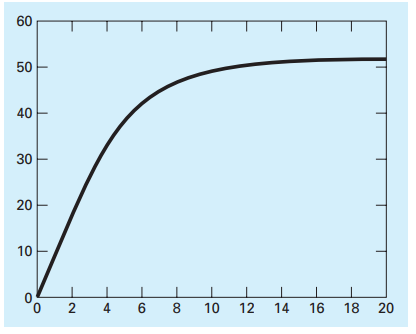
\includegraphics[width=0.50\textwidth]{fig_2_5_1}
   
\end{figure}

You can customize the graph a bit with commands such as the following:
\begin{lstlisting}[frame=none, numbers=none]
	>> title('Plot of v versus t')
	>> xlabel('Values of t')
	>> ylabel('Values of v')
	>> grid
\end{lstlisting}

\begin{figure}[H]
	\centering
	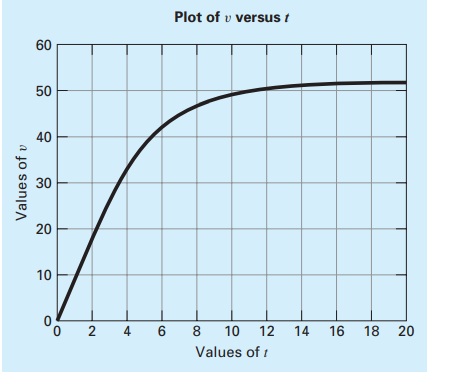
\includegraphics[width=0.50\textwidth]{fig_2_5_2}
   
\end{figure}

\begin{table}[H]
	\caption*{TABLE 2.2 Specifiers for colors, symbols, and line types.}
	\centering
	\begin{tabular}{l l l l l l }
		\hline

		Colors && Symbols&& Line Types&\\
		\hline
		Blue& b  &Point &.  &Solid& -\\
		Green& g& Circle& o&  Dotted& :\\
		Red& r &X-mark &x &Dashdot& -.\\
		Cyan &c &Plus &+ &Dashed& - -\\
		Magenta &m &Star& $ \ast $&&\\
		Yellow& y& Square& s&& \\
		Black& k &Diamond& d&& \\
		White& w &Triangle(down)& $\vee$ && \\
		&&Triangle(up) &$\wedge$ && \\
		&&Triangle(left)& <&& \\
		&&Triangle(right) &>&& \\
		&&Pentagram& p&& \\
		&&Hexagram& h&& \\
		\hline
	\end{tabular}	
\end{table}


The plot command displays a solid thin blue line by default. If you want to plot each
point with a symbol, you can include a specifier enclosed in single quotes in the plot 
function. Table 2.2 lists the available specifiers. For example, if you want to use open circles enter
\begin{lstlisting}[frame=none, numbers=none]
	>> plot(t, v, 'o')
\end{lstlisting}
You can also combine several specifiers. For example, if you want to use square green
markers connected by green dashed lines, you could enter
\begin{lstlisting}[frame=none, numbers=none]
	>> plot(t, v, 's--g')
\end{lstlisting}
You can also control the line width as well as the marker's size and its edge and face (i.e.,
interior) colors. For example, the following command uses a heavier (2-point), dashed,
cyan line to connect larger (10-point) diamond-shaped markers with black edges and
magenta faces:
\begin{lstlisting}[frame=none, numbers=none]
	>> plot(x,y,'--dc','LineWidth',2,...
	'MarkerSize',10,...
	'MarkerEdgeColor','k',...
	'MarkerFaceColor','m')
\end{lstlisting}
Note that the default line width is 1 point. For the markers, the default size is 6 point with
blue edge color and no face color.


MATLAB allows you to display more than one data set on the same plot. For example,
an alternative way to connect each data marker with a straight line would be to type
\begin{lstlisting}[frame=none, numbers=none]
	>> plot(t, v, t, v, 'o')
\end{lstlisting}

It should be mentioned that, by default, previous plots are erased every time the $plot$
command is implemented. The $hold on$ command holds the current plot and all axis properties 
so that additional graphing commands can be added to the existing plot. The $hold$
$off$ command returns to the default mode. For example, if we had typed the following
commands, the final plot would only display symbols:
\begin{lstlisting}[frame=none, numbers=none]
	>> plot(t, v)
	>> plot(t, v, 'o')
\end{lstlisting}


In contrast, the following commands would result in both lines and symbols being displayed:
\begin{lstlisting}[frame=none, numbers=none]
	>> plot(t, v)
	>> hold on
	>> plot(t, v, 'o')
	>> hold off
\end{lstlisting}
In addition to $hold$, another handy function is $subplot$, which allows you to split the
graph window into subwindows or panes. It has the syntax
\begin{lstlisting}[frame=none, numbers=none]
	>> plot(t, v, t, v, 'o')
\end{lstlisting}subplot(m, n, p)
This command breaks the graph window into an $m$-by-$n$ matrix of small axes, and selects
the p-th axes for the current plot.


We can demonstrate $subplot$ by examining MATLAB's capability to generate threedimensional plots. The simplest
 manifestation of this capability is the $plot3$ command
which has the syntax
\begin{lstlisting}[frame=none, numbers=none]
	plot3(x, y, z)
\end{lstlisting}
where $x, y,$ and z are three vectors of the same length. The result is a line in three-dimensional
space through the points whose coordinates are the elements of $x, y,$ and $z.$
Plotting a helix provides a nice example to illustrate its utility. First, let's graph a circle
with the two-dimensional $plot$ function using the parametric representation: $x = sin(t)$
and $y = cos(t)$. We employ the $subplot$ command so we can subsequently add the threedimensional plot.
\begin{lstlisting}[frame=none, numbers=none]
	>> t = 0:pi/50:10*pi;
	>> subplot(1,2,1);plot(sin(t),cos(t))
	>> axis square
	>> title('(a)')
\end{lstlisting}
As in Fig. 2.1a, the result is a circle. Note that the circle would have been distorted if we
had not used the axis square command.


Now, let's add the helix to the graph's right pane. To do this, we again employ a parametric representation:
 $x = sin(t)$, $y = cos(t)$, and $z = t$
 \begin{lstlisting}[frame=none, numbers=none]
	>> subplot(1,2,2);plot3(sin(t),cos(t),t);
	>> title('(b)')
\end{lstlisting}
The result is shown in Fig. 2.1b. Can you visualize what's going on? As time evolves,
the$ x$ and$ y$ coordinates sketch out the circumference of the circle in the $x-y$ plane in the
same fashion as the two-dimensional plot. However, simultaneously, the curve rises vertically as the z coordinate 
increases linearly with time. The net result is the characteristic
spring or spiral staircase shape of the helix.


There are other features of graphics that are useful—for example, plotting objects
instead of lines, families of curves plots, plotting on the complex plane, log-log or semilog
plots, three-dimensional mesh plots, and contour plots. As described next, a variety of resources are available
 to learn about these as well as other MATLAB capabilities.


\section{OTHER RESOURCES}


The foregoing was designed to focus on those features of MATLAB that we will be using
in the remainder of this book. As such, it is obviously not a comprehensive overview of all
of MATLAB's capabilities. If you are interested in learning more, you should consult one


\begin{figure}[H]
	\centering
	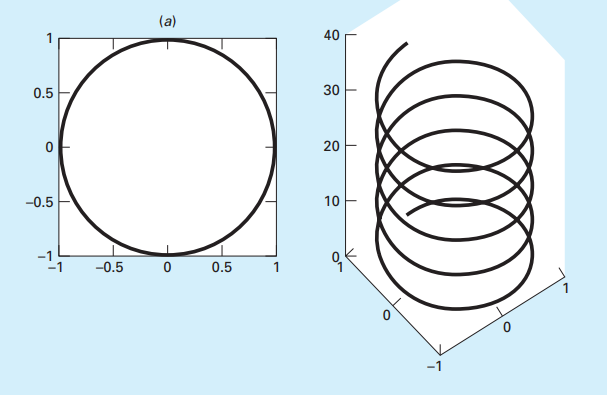
\includegraphics[width=0.75\textwidth]{fig_2_1}
   \caption{\textsf{A two-pane plot of (a) a two-dimensional circle and (b) a three-dimensional helix. }}
   \label{fig_2_1}
\end{figure}

of the excellent books devoted to MATLAB (e.g., Attaway, 2009; Palm, 2007; Hanselman
and Littlefield, 2005; and Moore, 2008).
Further, the package itself includes an extensive Help facility that can be accessed by
clicking on the Help menu in the command window. This will provide you with a number
of different options for exploring and searching through MATLAB's Help material. In addition, it provides access to a number of instructive demos.
As described in this chapter, help is also available in interactive mode by typing the
help command followed by the name of a command or function.
If you do not know the name, you can use the lookfor command to search the
MATLAB Help files for occurrences of text. For example, suppose that you want to find all
the commands and functions that relate to logarithms, you could enter
\begin{lstlisting}[frame=none, numbers=none]

	>> lookfor logarithm

\end{lstlisting}
and MATLAB will display all references that include the word logarithm.
Finally, you can obtain help from The MathWorks, Inc., website at www.mathworks
.com. There you will find links to product information, newsgroups, books, and technical
support as well as a variety of other useful resources.

\section{CASE STUDY. EXPLORATORY DATA ANALYSIS}


Background. Your textbooks are filled with formulas developed in the past by
renowned scientists and engineers. Although these are of great utility, engineers and scientists
often must supplement these relationships by collecting and analyzing their own data. Sometimes this leads to a new 
formula. However, prior to arriving at a final predictive equation, we
usually “play” with the data by performing calculations and developing plots. In most cases,
our intent is to gain insight into the patterns and mechanisms hidden in the data.


In this case study, we will illustrate how MATLAB facilitates such exploratory data
analysis. We will do this by estimating the drag coefficient of a free-falling human based on
Eq. (2.1) and the data from Table 2.1. However, beyond merely computing the drag
coefficient, we will use MATLAB's graphical capabilities to discern patterns in the data.
Solution. The data from Table 2.1 along with gravitational acceleration can be entered as

\begin{lstlisting}[frame=none, numbers=none]
	>> m=[83.6 60.2 72.1 91.1 92.9 65.3 80.9];
	>> vt=[53.4 48.5 50.9 55.7 54 47.7 51.1];
	>> g=9.81;
\end{lstlisting}

The drag coefficients can then be computed with Eq. (2.1). Because we are performing
element-by-element operations on vectors, we must include periods prior to the operators:
\begin{lstlisting}[frame=none, numbers=none]
	>> cd=g*m./vt.^2
	cd =
		0.2876 0.2511 0.2730 0.2881 0.3125 0.2815 0.3039
\end{lstlisting}
We can now use some of MATLAB's built-in functions to generate some statistics for the
results:
\begin{lstlisting}[frame=none, numbers=none]
	>> cdavg=mean(cd),cdmin=min(cd),cdmax=max(cd)
	cdavg =
		0.2854
	cdmin =
		0.2511
	cdmax =
		0.3125
\end{lstlisting}
Thus, the average value is 0.2854 with a range from 0.2511 to 0.3125 kg/m.
Now, let's start to play with these data by using Eq. (2.1) to make a prediction of the
terminal velocity based on the average drag:
\begin{lstlisting}[frame=none, numbers=none]
	>> vpred=sqrt(g*m/cdavg)
	vpred =
		53.6065 45.4897 49.7831 55.9595 56.5096 47.3774
		52.7338
\end{lstlisting}
Notice that we do not have to use periods prior to the operators in this formula? Do you
understand why?


We can plot these values versus the actual measured terminal velocities. We will also
superimpose a line indicating exact predictions (the 1:1 line) to help assess the results.


\begin{figure}[H]
	\centering
	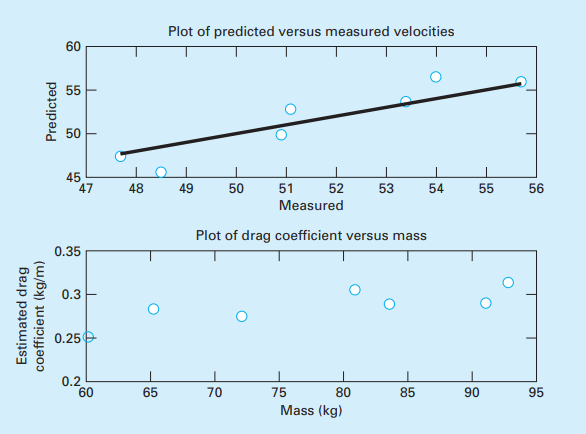
\includegraphics[width=0.75\textwidth]{fig_2_2}
   \caption{\textsf{Two plots created with MATLAB.}}
   \label{fig_2_2}
\end{figure}


Because we are going to eventually generate a second plot, we employ the subplot
command:
\begin{lstlisting}[frame=none, numbers=none]
	>> subplot(2,1,1);plot(vt,vpred,'o',vt,vt)
	>> xlabel('measured')
	>> ylabel('predicted')
	>> title('Plot of predicted versus measured velocities')
\end{lstlisting}


As in the top plot of Fig. 2.2, because the predictions generally follow the 1:1 line, you
might initially conclude that the average drag coefficient yields decent results. However,
notice how the model tends to underpredict the low velocities and overpredict the high.
This suggests that rather than being constant, there might be a trend in the drag coefficients.
This can be seen by plotting the estimated drag coefficients versus mass:
\begin{lstlisting}[frame=none, numbers=none]
	>> subplot(2,1,2);plot(m,cd,'o')
	>> xlabel('mass (kg)')
	>> ylabel('estimated drag coefficient (kg/m)')
	>> title('Plot of drag coefficient versus mass')
\end{lstlisting}

increases. Based on this result, you might conclude that your model needs to be improved.
At the least, it might motivate you to conduct further experiments with a larger number of
jumpers to confirm your preliminary finding.


In addition, the result might also stimulate you to go to the fluid mechanics literature and
learn more about the science of drag. As described previously in Sec. 1.4, you would discover that the parameter 
$c_d$ is actually a 
lumped drag coefficient that along with the true
drag includes other factors such as the jumper's frontal area and air density:

\begin{equation}
	\tag{2.2}
	c_d=\dfrac{C_D \rho A}{2}
\end{equation}

where $C_D$ = a dimensionless drag coefficient, $\rho$ = air density ($kg/m3$), and $A$ = frontal
area ($m^2$), which is the area projected on a plane normal to the direction of the velocity.


Assuming that the densities were relatively constant during data collection (a pretty
good assumption if the jumpers all took off from the same height on the same day), Eq. (2.2)
suggests that heavier jumpers might have larger areas. This hypothesis could be substantiated by measuring the frontal
 areas of individuals of varying masses.


The resulting plot, which is the bottom graph in Fig. 2.2, suggests that rather than
being constant, the drag coefficient seems to be increasing as the mass of the jumper

\bigskip
\section*{PROBLEMS}


\begin{multicols}{2}

			\textbf{2.1} Use the linspace function to create vectors identical to
	the following created with colon notation:
	\begin{enumerate}[label=(\alph*)]
		\item \texttt{t = 4:6:35}
		\item \texttt{x = -4:2}
	\end{enumerate}
	
	\textbf{2.2} Use colon notation to create vectors identical to the
	following created with the linspace function:
	\begin{enumerate}[label=(\alph*)]
		\item \texttt{v = linspace(-2,1.5,8)}
		\item \texttt{r = linspace(8,4.5,8)}
	\end{enumerate}
	

	\textbf{2.3} The command linspace(a, b, n) generates a row
	vector of n equally spaced points between a and b. Use
	colon notation to write an alternative one-line command to
	generate the same vector. Test your formulation for a = -3,
	b = 5, n = 6.


	\textbf{2.4} The following matrix is entered in MATLAB:
	\texttt{>> A=[3 2 1;0:0.5:1;linspace(6, 8, 3)]}
	\begin{enumerate}[label=(\alph*)]
		\item Write out the resulting matrix.
		\item Use colon notation to write a single-line MATLAB command to multiply the second row by the third column
		and assign the result to the variable $C$.
	\end{enumerate}
	

	\textbf{2.5} The following equation can be used to compute values
	of y as a function of x:

	$$y=be^{-ax}sin(bx)(0.012x^4-0.15x^3+0.075x^2+2.5x) $$

	where a and b are parameters. Write the equation for implementation with MATLAB, 
	where $a = 2$, $b = 5$, and $x$ is a
vector holding values from 0 to $ \pi $ /2 in increments of
$ \Delta $x = $ \pi $/40. Employ the minimum number of periods (i.e.,
dot notation) so that your formulation yields a vector for y.
In addition, compute the vector $z = y^2$ where each element
holds the square of each element of $y$. Combine $x, y,$ and $z$
into a matrix $w$, where each column holds one of the variables, and display w using the short g format. In addition,
generate a labeled plot of $y$ and $z$ versus x. Include a legend
on the plot (use help to understand how to do this). For $y$,
use a 1.5-point, dashdotted red line with 14-point, rededged, white-faced pentagram-shaped markers. For z, use a
standard-sized (i.e., default) solid blue line with standardsized, blue-edged, green-faced square markers.


\textbf{2.6} A simple electric circuit consisting of a resistor, a capacitor, and an inductor is depicted in Fig. P2.6. The charge
on the capacitor $q(t)$ as a function of time can be computed
as

$$q(t)=q_0e^{-Rt/(2L)}cos \left[\sqrt{ \dfrac{1}{LC}-\left(\dfrac{R}{2L} \right)^2 }t\right]$$


\begin{figure}[H]
	\centering
	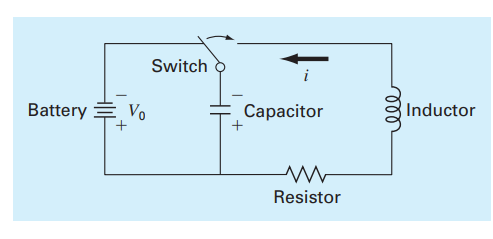
\includegraphics[width=0.40\textwidth]{fig_P2_6}
   \caption*{\textsf{FIGURE P2.6}}
   
\end{figure}

where t = time, $q_0$ = the initial charge, R = the resistance,
L = inductance, and C = capacitance. Use MATLAB to
generate a plot of this function from t = 0 to 0.8, given that
$q_0$ = 10, R = 60, L = 9, and C = 0.00005.


\textbf{2.7} The standard normal probability density function is a
bell-shaped curve that can be represented as

$$f(z)=\dfrac{1}{\sqrt{2\pi}}e^{-z^2/2} $$

Use MATLAB to generate a plot of this function from
$z = -5$ to 5. Label the ordinate as frequency and the abscissa as$ z$.


\textbf{2.8} If a force $F$ (N) is applied to compress a spring, its displacement x (m) can often be modeled by Hooke's law:

$$F=kx $$


where $k =$ the spring constant $(N/m)$. The potential energy
stored in the spring $U (J)$ can then be computed as


$$U=\dfrac{1}{2}kx^2 $$

Five springs are tested and the following data compiled:

\begin{tabular}{cccccc}
	\hline
	\textbf{F, N} &14 &18& 8 &9& 13\\
	\textbf{x, m}& 0.013 &0.020& 0.009& 0.010& 0.012\\
	\hline
	
\end{tabular}
Use MATLAB to store F and x as vectors and then compute
vectors of the spring constants and the potential energies.
Use the max function to determine the maximum potential
energy.


\textbf{2.9} The density of freshwater can be computed as a function
of temperature with the following cubic equation:


$$ \rho =5.5289x10^{-8}T_C^3-8.5016 \times 10^{-6}T_C^2 $$
$$+6.5622 \times 10^{-5}T_C+0.99987$$
where $\rho$ = density ($g/cm^3$
) and $T_C$ = temperature ($^{\circ} C$). Use
MATLAB to generate a vector of temperatures ranging from
32 F to 93.2 F using increments of 3.6 F. Convert this vector to degrees Celsius and then compute a vector of densities
based on the cubic formula. Create a plot of $\rho$ versus $T_C$ .
Recall that $T_C = 5/9(T_F - 32)$.


\textbf{2.10} Manning's equation can be used to compute the velocity of water in a rectangular open channel:
where $U$ = velocity (m/s), $S$ = channel slope, $n$ = roughness
coefficient, $B$ = width (m), and $H$ = depth (m). The following data are available for five channels:


\begin{tabular}{cccc}
	\hline
	\textbf{n}&\textbf{S}&\textbf{B}&\textbf{H}\\
	\hline
		0.035 &0.0001 &10 &2\\
		0.020 &0.0002 &8 &1\\
		0.015 &0.0010 &20 &1.5\\
		0.030 &0.0007 &24 &3\\
		0.022 &0.0003 &15 &2.5\\

	\hline
\end{tabular}


Store these values in a matrix where each row represents one
of the channels and each column represents one of the parameters. Write a single-line MATLAB statement to compute a
column vector containing the velocities based on the values
in the parameter matrix.


\textbf{2.11} It is general practice in engineering and science that
equations be plotted as lines and discrete data as symbols.
Here are some data for concentration $(c)$ versus time $(t)$ for
the photodegradation of aqueous bromine:


\begin{tabular}{ccccccc}
	\hline

	\textbf{t, min} &10 &20 &30 &40 &50 &60\\
	\textbf{c, ppm} &3.4 &2.6 &1.6 &1.3 &1.0 &0.5\\

	\hline
\end{tabular}


These data can be described by the following function:

$$ c=4.84e^{-0.034t}$$

Use MATLAB to create a plot displaying both the data
(using diamond-shaped, filled-red symbols) and the function
(using a green, dashed line). Plot the function for t = 0 to
70 min.


\textbf{2.12} The \texttt{semilogy} function operates in an identical fashion
to the \texttt{plot} function except that a logarithmic (base-10) scale
is used for the y axis. Use this function to plot the data and
function as described in Prob. 2.11. Explain the results.


\textbf{2.13} Here are some wind tunnel data for force (F) versus
velocity $(v)$:

	\begin{flushleft}
	\begin{small}
		
	
	\begin{tabular}{ccccccccc}
		\hline
		\textbf{v, m/s} &10& 20& 30 &40& 50 &60 &70 &80	\\
		\textbf{F, N} &25 &70 &380 &550 &610 &1220 &830 &1450\\
		\hline
	
	\end{tabular}
\end{small}
\end{flushleft}



These data can be described by the following function:


$$F=0.2741v^{1.9842} $$

Use MATLAB to create a plot displaying both the data (using
circular magenta symbols) and the function (using a black
dash-dotted line). Plot the function for $v = 0$ to 100 m/s and
label the plot's axes.


\textbf{2.14} The \texttt{loglog} function operates in an identical fashion
to the \texttt{plot} function except that logarithmic scales are used
for both the x and y axes. Use this function to plot the data
and function as described in Prob. 2.13. Explain the results.



\textbf{2.15} The Maclaurin series expansion for the cosine is

$$cosx = 1 - \dfrac{x^2}{2!}+ \dfrac{x^4}{4!}- \dfrac{x^6}{6!}+ \dfrac{x^8}{8!}- \ldots $$


Use MATLAB to create a plot of the sine (solid line) along
with a plot of the series expansion (black dashed line) up
to and including the term x8/8!. Use the built-in function
factorial in computing the series expansion. Make the
range of the abscissa from $x = 0$ to $3\pi /2$.


\textbf{2.16} You contact the jumpers used to generate the data in
Table 2.1 and measure their frontal areas. The resulting
values, which are ordered in the same sequence as the
corresponding values in Table 2.1, are
\begin{flushleft}
	\begin{scriptsize}
	\begin{tabular}{cccccccc}
		\hline
		\textbf{$A, m^2$} &0.455 &0.402 &0.452& 0.486 &0.531 &0.475 &0.487\\
		\hline
		
	\end{tabular}
\end{scriptsize}
\end{flushleft}


\begin{enumerate}[label=(\alph*)]
	\item If the air density is $\rho$ = 1.223 $kg/m^3$
	, use MATLAB to
	compute values of the dimensionless drag coefficient $C_D$.
	\item Determine the average, minimum and maximum of the
	resulting values.
	\item Develop a stacked plot of$ A$ versus $m$ (upper) and $C_D$
	versus m (lower). Include descriptive axis labels and
	titles on the plots.
\end{enumerate}


\textbf{2.17} The following parametric equations generate a conical
helix
\[ \begin{array}{lll}
	x &= &t cos(6t)\\
	y &= &t sin(6t)\\
	z &= &t\\

	
\end{array} \]

Compute values of $x, y,$ and z for $t = 0$ to $6\pi $with
$\Delta $= $\pi/64$. Use \texttt{subplot} to generate a two-dimensional
line plot (red solid line) of ($x, y$) in the top pane and a threedimensional line plot (cyan solid line) of (x, y, z) in the
bottom pane. Label the axes for both plots.


\textbf{2.18} Exactly what will be displayed after the following
MATLAB commands are typed?
\begin{enumerate}[label=(\alph*)]
		

	\item 
	\begin{lstlisting}[frame=none, numbers=none]
		>> x = 5;
		>> x ^ 3;
		>> y = 8 - x
	\end{lstlisting}
	\item 
	\begin{lstlisting}[frame=none, numbers=none]
		>> q = 4:2:12;
		>> r = [7 8 4; 3 6 -5];
		>> sum(q) * r(2, 3) 
	\end{lstlisting}
\end{enumerate}

\textbf{2.19} The trajectory of an object can be modeled as

$$y=(tan\theta_0  )x-\dfrac{g}{2v_0^2cos^2\theta_0 }x^2+y_0$$


where $y =$ height (m), $\theta_0 =$ initial angle (radians), $x =$
horizontal distance (m), $g$ = gravitational acceleration($= 9.81 m/s^2$
),$ v_0$ = initial velocity (m/s), and $y_0 =$ initial
height. Use MATLAB to find the trajectories for$ y_0 = 0$ and
$v_0 = 28 m/s$ for initial angles ranging from 15 to 75$^{\circ}$ in increments of 15$^{\circ}$. Employ a 
range of horizontal distances
from $x = 0$ to 80 m in increments of 5 m. The results should
be assembled in an array where the first dimension (rows)
corresponds to the distances, and the second dimension
(columns) corresponds to the different initial angles. Use
this matrix to generate a single plot of the heights versus
horizontal distances for each of the initial angles. Employ a
legend to distinguish among the different cases, and scale
the plot so that the minimum height is zero using the texttt{axis}
command.

\textbf{2.20} The temperature dependence of chemical reactions can
be computed with the Arrhenius equation:

$$k=Ae^{-E/RT_a}$$

where $k =$ reaction rate ($s^{-1}$), $A =$ the preexponential (or frequency) factor, 
$E =$ activation energy (J/mol), $R = $gas constant [8.314 J/(mole $\cdot$  K)], and $T_a =$ absolute temperature
(K). A compound has $E = 1 \times  105$ J/mol and $A = 7 \times 1016$.
Use MATLAB to generate values of reaction rates for
temperatures ranging from 253 to 325 K. Use texttt{subplot} to
generate a side-by-side graph of (a) k versus Ta (green line)
and (b) log10 k (red line) versus 1/Ta. Employ the texttt{semilogy}
function to create (b). Include axis labels and titles for both
subplots. Interpret your results.


\textbf{2.21} Figure P2.21a shows a uniform beam subject to a linearly increasing distributed load. As depicted in Fig. P2.21b,
deflection y (m) can be computed with

$$y=\dfrac{\omega_0}{120EIL}(-x^5+2L^2x^3-L^4x)$$

where E = the modulus of elasticity and $I =$ the moment of
inertia ($m^4$). Employ this equation and calculus to generate
MATLAB plots of the following quantities versus distance
along the beam:

\begin{enumerate}[label=(\alph*)]
	\item displacement ($y$), 
	\item slope [$\theta(x) = dy/dx$], 


\begin{figure}[H]
	\centering
	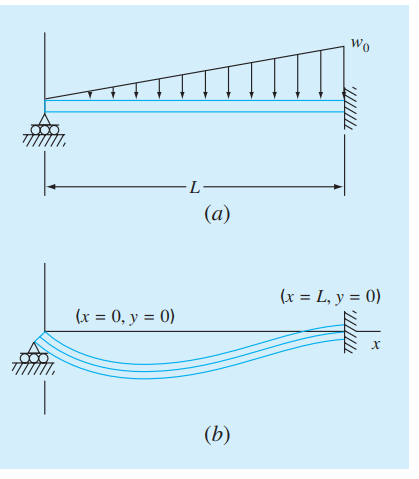
\includegraphics[width=0.40\textwidth]{fig_P2_21}
   \caption*{\textsf{FIGURE P2.21}}
   \label{fig_P2_6}
\end{figure}
\item moment [$M(x) = EId^2 y/dx^2$],
\item shear [$V(x) = EId^3 y/dx^3$], and

\item loading [$w(x) = -EId^4 y/dx^4$].
Use the following parameters for your computation:
$L = 600 cm, E = 50,000 kN/cm2$ , $I = 30,000 cm^4$,

$\omega_0 = 2.5 kN/cm$, and $\Delta x = 10 cm$. Employ the texttt{subplot}
function to display all the plots vertically on the same page
in the order (a) to (e). Include labels and use consistent MKS
units when developing the plots.
\end{enumerate}

\textbf{2.22} The butterfly curve is given by the following parametric equations:

$$x = sin(t)\left( e^{\cos t} - 2 \cos 4t - \sin^5 \dfrac{t}{12} \right)$$

$$y = \cos(t)\left( e^{\cos t} - 2 \cos 4t - \sin^5 \dfrac{t}{12} \right)$$

Generate values of $x$ and $y$ for values of$ t$ from 0 to 100 with
$\Delta t = 1/16$. Construct plots of (a) $x$ and $y $versus $t$ and (b) $y$
versus $x$. Use subplot to stack these plots vertically and
make the plot in (b) square. Include titles and axis labels on
both plots and a legend for (a). For (a), employ a dotted line
for $y$ in order to distinguish it from $x$.


\textbf{2.23} The butterfly curve from Prob. 2.22 can also be represented in polar coordinates as



$$r= e^{sin \theta}-2\cos(4\theta )- \sin^5 \left(\dfrac{2\theta - \pi }{24} \right) $$

Generate values of $r$ for values of $\theta$ from 0 to $8\pi$ with
$\Delta\theta = \pi/32$. Use the MATLAB function \texttt{polar} to generate
the polar plot of the butterfly curve with a dashed red line.
Employ the MATLAB Help to understand how to generate
the plot.



\end{multicols}


\end{document}

